\documentclass[../../FisicaTeorica.tex]{subfiles}
\begin{document}


\section{Paradosso Einstein-Podolski-Rosen (1935)}
\begin{comment}
\vspace{-1em}
\begin{center}
    \small{(19/12/2018)}
\end{center}
\end{comment}

\textbf{Disclaimer.} Ci occuperemo in questa parte degli aspetti \textit{paradossali} e \text{\textit{filosofici}} della \MQ, che potrebbero far dubitare della sua validità o completezza. Si tenga conto del fatto che finora \textbf{nessun esperimento} contraddice la \MQ, su cui anzi si basano gran parte delle tecnologie più recenti.\\

\subsection{Realismo e controfattualità}
Prima di dedicarci ad analizzare gli aspetti \textit{fisici} del paradosso EPR, è necessario dare qualche definizione di carattere filosofico, esplicitando le \q{assunzioni inconsce} che vengono fatte nell'analisi scientifica. Solo in questo modo sarà possibile apprezzare appieno la natura \textit{paradossale}, nel senso etimologico di \q{contro l'esperienza comune}, dell'esperimento proposto da Einstein-Podolsky-Rosen nel 1935.\\

Con \textbf{realismo scientifico}\marginpar{Realismo scientifico} intendiamo la corrente filosofica, generalmente condivisa nella nostra società, che la conoscenza scientifica sia \textbf{rigorosa}, \textbf{oggettiva} e trovi \textbf{corrispondenza} con la realtà tramite esperimenti, e che la scienza ci dia informazioni sulle cose che esistono, non solo sugli oggetti di cui abbiamo percezione diretta tramite i sensi, ma anche su oggetti che non percepiamo direttamente ma compaiono nelle teorie, come \textit{atomi}, \textit{elettroni}, etc. (che, in principio, non sono \q{osservabili con gli occhi}).\\
All'opposto, l'\textbf{antirealismo scientifico}\marginpar{Strumentalismo} (o \textit{strumentalismo}) è la corrente filosofica che ritiene che le teorie scientifiche siano solo \textit{strumenti per predire i fenomeni}, ma non per descrivere il mondo come realmente è. Anzi, il mondo esterno potrebbe \q{non esistere}, o comunque non avremmo alcun accesso certo ad esso\footnote{CFR l'esperimento mentale del \q{brain in a vat}}.\\

Realismo e strumentalismo sono due visioni \textit{metafisiche}, nel senso che riguardano principalmente l'\textit{attitudine} di uno scienziato nel discutere una teoria. Per un realista gli \textit{elettroni} \q{esistono}, cioè \q{sono veri}, e hanno le proprietà (carica, massa, spin, etc.) date dalla teoria. Ogni nuova teoria fisica, perciò, non è altro che un'immagine \q{più dettagliata} di come l'universo \textit{è} realmente. Per uno strumentalista, gli \q{elettroni} sono solo un utile concetto - un nome da associare a formule matematiche che consentono di spiegare con precisione i fenomeni che percepiamo. Si può dire che un realista sia concentrato su come l'universo \textit{è}, indipendentemente da ogni cosa, mentre uno strumentalista, notando che possiamo percepire ogni cosa solo attraverso i sensi, e quindi da una prospettiva decisamente \textit{biased}, si limita a studiare le \textit{interazioni} tra universo e mente umana. Per un realista un albero che cade in mezzo ad una foresta senza che nessuno lo senta \textit{fa rumore}, mentre per uno strumentalista non ha senso porsi il problema dell'esito di una misura senza che essa sia stata svolta.\\

Se realismo e strumentalismo sono essenzialmente materia di preferenza personale, non è detto che i \textit{framework} da esse generati siano equivalenti.\\
In particolare, un realista tende - quasi inconsciamente - ad assumere una proprietà \textit{epistemologica} (cioè legata alla natura del conoscere) detta \textbf{definitezza controfattuale}\footnote{In inglese: counterfactual definiteness} (CFD)\marginpar{Definitezza controfattuale}. L'idea della CFD è che la realtà \q{esista} mentre non la si osserva, e che porsi domande su esiti di misure \textit{non svolte} di \q{proprietà reali} abbia senso. Se la Luna è \textit{reale}, allora continua ad \textit{esistere} anche se nessuno può vederla perché un cataclisma ha sterminato l'umanità intera.\\

Per applicare la definizione di CFD è necessario definire un \textit{modo} per riconoscere gli elementi della \textbf{realtà oggettiva}, che sono in principio distinti dai \textbf{concetti fisici} utilizzati da una teoria scientifica per spiegarli. A tal proposito, ci accontenteremo della seguente \textbf{condizione sufficiente}: \textit{se senza disturbare in nessun modo un sistema possiamo prevedere con certezza\marginpar{Elemento di realtà oggettiva} (cioè con probabilità unitaria) il valore di una quantita fisica $A$, allora esiste un elemento di realtà fisica corrispondente a questa quantità fisica}.\\
Accettando la CFD, possiamo aggiungere che $A$, essendo reale, avrebbe avuto lo stesso valore anche se la misura non fosse stata eseguita.\\
In altre parole, per la CFD le \textit{proprietà reali} di un sistema (date per esempio dalla condizione di sopra) hanno \textit{un unico valore ben definito} in ogni istante: per esempio la massa di un elettrone è \textit{definita} anche se non la stiamo misurando.\\


Il problema del paradosso EPR sta proprio nel fatto che la CFD, ingenuamente accettata in ottica realista e perfettamente compatibile con la \MC, non è rispettata in \MQ. Tale inaspettata conseguenza è stata effettivamente verificata sperimentalmente con ottima precisione\footnote{\url{https://www.nature.com/articles/nature15759}}.


\subsection{I principi del paradosso EPR}
Il paradosso EPR sorge combinando due principi \textit{ragionevoli} e comunemente assunti:
\begin{itemize}
\item \textbf{Principio di realtà} $\mathcal{R}$: Se, senza intervenire su un dato sistema, è possibile prevedere con certezza (cioè con probabilità unitaria) il valore di una grandezza fisica, a questa corrisponde una \textbf{proprietà oggettiva} del sistema, cioè una proprietà indipendente da eventuali osservatori esterni che (CFD) avrebbe lo stesso valore anche se la misura non fosse stata effettuata.\\

Per esempio, se in \MC misuriamo $(q,p)$, sappiamo che la particella avrebbe avuto posizione e momento $(q,p)$ anche se non fossero stati misurati, poiché si può assumere \textit{idealmente} che il processo di misura \textit{non disturbi} il sistema.\\
In \MQ ciò è applicabile \textit{solo agli autostati}. Ad esempio, supponiamo che lo stato di spin sia dato da $\ket{+}$ autostato di $S_z$ di autovalore $+\hbar/2$, allora diremo che l'elettrone \q{ha} spin $\hbar/2$, indipendentemente dal fatto che lo misuriamo o meno, poiché questa è una \textit{proprietà oggettiva} di quell'elettrone.

\textbf{Nota}: Già in questa prima accezione notiamo come la \MQ differisca dalla \MC, dato che nella prima possiamo  applicare l'idea di \textit{proprietà oggettiva} esclusivamente agli \textit{autostati}, e non a tutti gli stati.
\item \textbf{Principio di località} \marginpar{Località}(alla Einstein) $\mathcal{L}$.\\
Dati due sistemi fisici e supposto che durante un certo intervallo di tempo $\Delta t$ essi rimangano \textit{isolati} tra loro (cosa realizzata in relatività se la distanza tra di essi è più grande di $c\Delta t$), allora l'evoluzione delle proprietà fisiche (determinate dagli \q{elementi di realtà}) di uno di essi durante tale intervallo di tempo non può essere influenzata da operazioni eseguite sull'altro.

In parole povere, il principio di località afferma che ogni oggetto è influenzato direttamente solo dalle sue immediate vicinanze. L'idea è che ogni interazione abbia una velocità \textit{finita} (che è $\leq c$ per la relatività), e perciò perturbare un oggetto $A$ non può influenzare istantaneamente un altro oggetto $B$ posto ad una certa distanza da esso. Per esempio, se il Sole esplodesse, la Terra non subirebbe alcun effetto per circa $8$ minuti, poiché tale è il tempo impiegato dalla luce per percorrere la distanza Sole-Terra, e per $\mathcal{L}$ nessuna interazione può propagarsi più velocemente di $c$. Analogamente, spingere su una ipotetica barra lunga $1$ anno luce produce un'onda di compressione su di essa che si propaga alla velocità del suono, che è sicuramente $< c$, e perciò l'effetto della spinta giunge all'altro estremo non istantaneamente.\\
La località è molto importante sia per garantire che la causalità sia rispettata (se la velocità di ogni segnale è limitata è automaticamente impossibile una \textit{macchina del tempo} che comunica con il passato), che per \textit{semplificare} la trattazione dei sistemi fisici. Nel corso di un esperimento, infatti, vorremmo dover considerare solo un numero finito di corpi che possono interagire con l'apparato in questione, e non rassegnarci a dover tener conto di \textit{tutto l'universo} - cosa che ha il potenziale di negare buona parte delle capacità predittive della fisica.
\end{itemize}

%[TO DO]Citare Nicrosini

\subsection{Versione classica di EPR}
Verifichiamo la compatibilità di $\mathcal{L}$ + $\mathcal{R}$ in \MC con un sistema \textit{analogo classico} dell'EPR.
\begin{figure}[H]
\centering
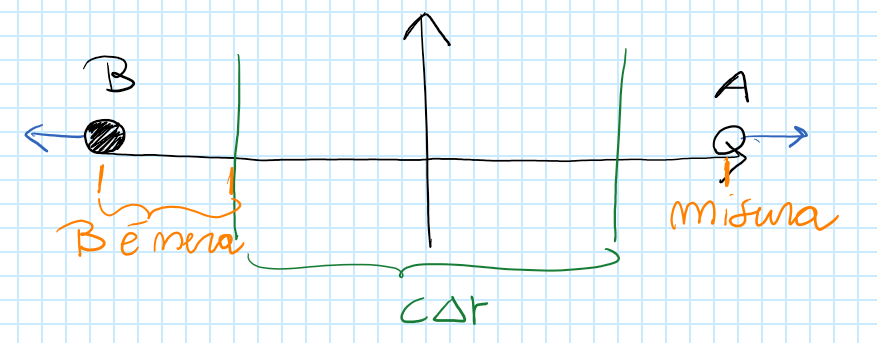
\includegraphics[scale=0.4]{Immagini/19_12/image002.png}
\caption{Schema dell'analogo classico del paradosso EPR}
\end{figure}

Consideriamo un insieme di coppie di palle classiche che si muovono una verso destra (palle $A$) e una verso sinistra (palle $B$), e di cui sappiamo che una è bianca e l'altra è nera, ma non sappiamo \textit{quale}, e la distribuzione dei colori è casuale.\\
$A$ e $B$ partono dall'origine del sdr del laboratorio a $t=0$. Per semplicità, consideriamo che $A$ e $B$ possano interagire fino ad un certo tempo $T$, dopodiché, per $t>T$, data la loro distanza, siano considerabili indipendenti (ossia si trovino a distanza di tipo \textit{spazio} relativamente alla scala temporale $\Delta t$ dell'esperimento). Per esempio potremmo aspettare che $A$ e $B$ si trovino a $1$ anno luce di distanza, per cui ogni modifica fatta su $A$ possa influenzare $B$ solo dopo un anno, ossia molto dopo la conclusione dell'esperimento.\\
A $T+t_0$, dove $t_0$ è dell'ordine di $\Delta t$ (e quindi $\ll$ 1 anno), osserviamo $A$, che supponiamo essere bianca. Poiché sappiamo che, per ipotesi, osservando $A$ e $B$ simultaneamente (rispetto al sdr del laboratorio), una è nera e l'altra è bianca, deduciamo che $B$ a $T+t_0$ deve essere \textbf{nera}.\\
Abbiamo allora ottenuto una misura del colore di $B$ senza perturbarla in alcun modo. Per $\mathcal{R}$ si ha che il \textit{colore} è una proprietà oggettiva di $B$, intesa come \textit{reale}. Segue allora, per la CFD, che $B$ deve avere un colore \textit{definito} ad ogni istante: dato che stiamo parlando di un qualcosa di \q{reale}, non può assumere proprietà contraddittorie!
Per $t<T+t_0$ abbiamo allora due possibilità mutualmente esclusive:
\begin{itemize}
\item $B$ era bianca
\item $B$ era nera
\end{itemize}
Il principio di località $\mathcal{L}$ ci porta a scartare la prima. Se $B$ fosse stata bianca prima di $T_0+t$, allora significa che la misura di $A$ ha modificato una proprietà fisica di $B$, nonostante $A$ e $B$ fossero \textit{separate} e \textit{non interagenti}, ma questo è escluso da $\mathcal{L}$. Deve allora essere che, per $t<T + t_0$, $B$ era nera.\\
In realtà, prima di $T$ ammettiamo la possibilità di interazioni tra $A$ e $B$, che possono modificarne i rispettivi stati. Perciò, da $\mathcal{R} + \mathcal{L}$ deduciamo che, data la misura di $A$ bianca a $T+t_0$, $B$ deve essere nera almeno per $T < t < T+t_0$, dove $T$ è il tempo dopo il quale $A$ e $B$ sono considerabili \textit{non interangenti} nella scala temporale dell'esperimento.\\


Tutto ciò non stupisce. L'indeterminatezza iniziale è di \q{tipo classico}, nel senso che deriva da un'ignoranza dello sperimentatore: lo stato iniziale del sistema non era infatti di conoscenza massimale. Dopo la misura di $A$, e la relativa deduzione per $B$ tramite $\mathcal{R}+\mathcal{L}$, la nostra conoscenza del sistema si è accresciuta, compatibilmente con una \textbf{realtà preesistente}.\\
Possiamo perciò dire che la \MC è compatibile con il \textbf{realismo locale} ($\mathcal{R}+\mathcal{L}$). 
\begin{comment}
\textbf{Nota}: non possiamo dire nulla sul colore di $A$ \textit{prima} della sua misura, dato che potenzialmente la misura potrebbe aver \textit{disturbato} tale proprietà, ma per induzione sappiamo con certezza il colore di $B$, indipendentemente che la misuriamo o meno.\\
\end{comment}


\subsection{Versione quantistica di EPR}
Passiamo ora alla versione quantistica dell'esperimento, in cui al posto di palle consideriamo elettroni, e invece del colore lo \textit{spin}.\\
Sia dato un numero $N\gg1$ di particelle di spin $0$ che decadono a $t=0$ in coppie di particelle di spin $1/2$  in uno stato \textit{entangled} di \textit{singoletto}, ossia tale che:
\begin{align*}
S^{tot}=0\qquad S_z^{tot}=0
\end{align*}
Che deriva dalla \textit{conservazione dello spin} (analoga all'usuale conservazione del momento angolare).\\
Perciò le $N$ coppie di elettroni assumono a $t=0$ lo stato puro:
\begin{align*}
\ket{\psi}=\frac{1}{\sqrt{2}}\left(\ket{+}_A\ket{-}_B - \ket{-}_A\ket{+}_B\right)
\end{align*}
dove con $\ket{+}$ e $\ket{-}$ denotiamo gli autostati, rispettivamente della particella $A$ e $B$, dell'operatore $S_z$.\\
Consideriamo una di queste coppie, dove indichiamo con $A$ l'elettrone emesso verso destra, e con $B$ quello verso sinistra.\\
%disegnetto

Ad un certo istante $t_0 > 0$, i supporti delle funzioni d'onda spaziali dei due elettroni si trovano a una distanza tale da far sì che non possano interagire tra loro senza violare $\mathcal{L}$.\\
Dopodiché a $t_1>t_0$ l'osservatore $A$ misura lo spin $S_z^A$. Dato che gli autostati di $A$ sono una combinazione \textit{in parti uguali} di $\ket{+}_A$ e $\ket{-}_A$, $A$ osserverà per circa metà delle coppie uno spin $\hbar/2$, e per un'altra metà uno spin $-\hbar/2$.\\
Nel primo caso, per il postulato di proiezione di Von Neumann, lo stato di spin delle coppie dopo la misura diventa:
\begin{align*}
\ket{\psi'}=\left(\ket{+}_A \bra{+}_A\otimes \bb{I}_B\right) \ket{\psi} = \frac{1}{\sqrt{2}}\ket{+}_A \ket{-}_B
\end{align*}
che, una volta normalizzato, corrisponde allo stato puro:
\begin{align*}
\ket{\psi'} = \ket{+}_A \ket{-}_B
\end{align*}

Siamo allora \textit{certi} che se facessimo una misura di $S_z^B$ troveremmo $-\hbar/2$, visto che $\ket{\psi'}$ è \textit{autostato} di $S_z^B$. Sappiamo che la misura su $A$ non può aver disturbato $B$. Infatti, per ipotesi di \textit{separabilità}\footnote{Questa ipotesi era contenuta implicitamente nel primo enunciato di $\mathcal{L}$, e la esplicitiamo qui per completezza. Si noti che, senza separabilità, non sarebbe possibile parlare di località.} di $A$ e $B$, nel senso che i due elettroni hanno \q{realtà distinte} e non sono un unico oggetto, ha senso parlare di una misura solo su uno di essi ($A$) e per località ogni perturbazione non può propagarsi istantaneamente. Si verifica allora la \textit{condizione sufficiente} di $\mathcal{R}$,
da cui segue che lo spin è una \textit{proprietà oggettiva} di $B$.\\
Per $\mathcal{L}$, la misura appena fatta non può aver prodotto una proprietà di $B$, che quindi doveva essere già così, almeno dal momento in cui $A$ e $B$ non potevano più interagire. Perciò, per $t_0 < t \leq t_1$ sappiamo che $B$ aveva uno \textbf{spin definito}, e pari a $-\hbar/2$.\\
Si ha perciò che la coppia considerata si trova nello stato $\ket{\psi}$ per $t\in [0,t_0]$, e in $\ket{\psi'}$ per $t \in [t_0,t_1]$.\\

In generale, ripetendo l'esperimento più volte, si avrà che l'esito della misura a $t_1$, da cui deduciamo per $\mathcal{R}+\mathcal{L}$ lo stato $\ket{\psi'}$ per $t\in[t_0,t_1]$, sarà equamente $+\hbar/2$ o $-\hbar/2$. Ciò significa che, per molti esperimenti, lo stato per $t\in[t_0,t_1]$ sarà una \q{miscela} delle due possibilità $\ket{\psi'_+} = \ket{+}_A\ket{-}_B$ e $\ket{\psi'_-}=\ket{-}_A\ket{+}_B$, ciascuna con probabilità $1/2$, ossia uno \textbf{stato misto} $\rho$: 
\begin{align*}
\rho &= \frac{1}{2}\ket{\psi'_+}\bra{\psi'_+} + \frac{1}{2}\ket{\psi'_-}\bra{\psi'_-}=\\
&=
 \frac{1}{2}\left( \ket{+}_A \prescript{}{A}{\bra{+}}
\otimes \ket{-}_B \prescript{}{B}{\bra{-}} 
\right)
+ \frac{1}{2} \left(\ket{-}_A \prescript{}{A}{\bra{-}}\otimes \ket{+}_{B}\prescript{}{B}{\bra{+}}\right)
\end{align*}

Il problema sorge osservando che, per $t \in [0,t_1]$, la misura non è stata ancora effettuata (lo sarà a $t_1$), e perciò lo stato del sistema \textit{non è collassato} per proiezione di von Neumann, e deve essere $\ket{\psi(t)}$ dato dall'evoluzione unitaria:
\begin{align*}
\ket{\psi(t)} = \exp\left(-\frac{i}{\hbar}tH\right)\ket{\psi}
\end{align*}
Si dimostra che l'evoluzione unitaria non può portare uno stato inizialmente puro $\ket{\psi}$ ad uno stato misto $\rho$.\\
Infatti, partendo da uno stato puro generico $\ket{\psi}\bra{\psi}$ e calcolandone l'evoluto temporale ($U\ket{\psi}=\ket{\psi(t)}$) si ottiene sempre uno stato puro:
\begin{align*}
U\ket{\psi}\bra{\psi}U^\dag = \ket{\psi(t)}\bra{\psi(t)}
\end{align*}

Perciò affermare (grazie a $\mathcal{R}+\mathcal{L}$) che per $t\in [t_0,t_1]$ lo stato della coppia è $\rho$ è incompatibile con l'evoluzione unitaria dello stato iniziale $\ket{\psi}$, che prevederebbe, sempre per $t\in[t_0, t_1]$ uno stato $\ket{\psi(t)}$ fondamentalmente diverso.\\

Si ha infatti che $\rho$ e $\ket{\psi(t)}$ producono valori medi differenti per misure di correlazione di osservabili che non sono diagonali nella base $\{\ket{+},\ket{-}\}$ degli autostati di $S_z$ utilizzata per definire $\ket{\psi(t)}$ e $\rho$.\\
Possiamo usare, per esempio, $S_x$, dato che $[S_x, S_z] \neq 0$ e perciò sicuramente $S_x$ non è diagonale nella base degli autoket di $S_z$. In particolare, l'autoket di autovalore $\hbar/2$ di $S_x$ è dato da:
\begin{align}
\ket{+}_x = \frac{1}{\sqrt{2}}(\ket{+}+\ket{-})
\label{eqn:spinxz}
\end{align}
Una misura di correlazione di $S_x$ consiste nel misurare \textit{contemporaneamente} $S_x$ su entrambe le particelle $A$ e $B$ al tempo $t \in [t_0, t_1]$.\\
Con una scelta opportuna della fase iniziale, $\ket{\psi(t)}=\ket{\psi}$, che riscriviamo come:
\begin{align}
\ket{\psi} = \frac{1}{\sqrt{2}}\left(\hlc{Yellow}{\ket{+}_A\ket{-}_B }- \hlc{SkyBlue}{\ket{-}_A\ket{+}_B}\right) = \frac{1}{\sqrt{2}}(\hlc{Yellow}{\ket{\psi_1}}-\hlc{SkyBlue}{\ket{\psi_2}})
\label{eqn:def-psip}
\end{align}
Denotiamo con $P_+$ il proiettore sull'autospazio di $S_x^A \otimes S_x^B$ di autovalore $\hbar/2, \hbar/2$ dato da:
\begin{align*}
P_+ &= \ket{+}_x^A \prescript{A}{x}{\bra{+}} \otimes \ket{+}_x^B \prescript{B}{x}{\bra{+}} =\\
&\underset{(\ref{eqn:spinxz})}{=} \left(\frac{\ket{+}_A+\ket{-}_A}{\sqrt{2}}\frac{\prescript{}{A}{\bra{+}+\prescript{}{A}{\bra{-}}}}{\sqrt{2}}
\right) \otimes
\left(
\frac{\ket{+}_B + \ket{-}_B}{\sqrt{2}}\frac{\prescript{}{B}{\bra{+}+\prescript{}{B}{\bra{-}}}}{\sqrt{2}}
\right) =\\
&= \frac{1}{2}\left[\ket{+}\bra{+}+\ket{-}\bra{-}+\ket{+}\bra{-}+\ket{-}\bra{+}\right] \otimes \frac{1}{2}\left[\ket{+}\bra{+}+\ket{-}\bra{-}+\ket{+}\bra{-}+\ket{-}\bra{+}\right]
\end{align*}
La probabilità cercata si ottiene allora da:
\begin{align} \nonumber
W_{\ket{\psi}}^{S_x^A S_x^B} &= \norm{P_+ \ket{\psi}}^2 \underset{(\ref{eqn:def-psip})}{=} \norm{P_+ \frac{1}{\sqrt{2}}(\ket{\psi_1} - \ket{\psi_2} }^2 =\\
&\underset{(a)}{=} \frac{1}{2}\norm{P_+ \ket{\psi_1}}^2 + \frac{1}{2}\norm{P_+ \ket{\psi_2}}^2 - \frac{1}{2}\bra{\psi_2}P_+ \ket{\psi_1}-\frac{1}{2}\bra{\psi_1}P_+\ket{\psi_2} \label{eqn:prob-p}
\end{align}
dove in (a) abbiamo sviluppato la norma, usando la linearità di $P_+$.\\
Otteniamo:
\begin{align*}
\norm{P_+\ket{\psi_1}}^2 &= \left|
\frac{1}{2}[\ket{+}_A+\ket{-}_A] \otimes \frac{1}{2}[\ket{+}_B+\ket{-}_B]
\right|^2 = \frac{1}{4}(1+1)\frac{1}{4}(1+1) =\frac{1}{4}\\
\bra{\psi_1}P_+ \ket{\psi_2} &= \bra{\psi_1} \left(\frac{1}{2}[\ket{+}_A+\ket{-}_A] \otimes \frac{1}{2}[\ket{+}_B+\ket{-}_B] \right)
= \frac{1}{2}\frac{1}{2} = \frac{1}{4}
\end{align*}
Per simmetria (notando che $P_+$ non cambia per scambio di particelle) si ha $\norm{P_+\ket{\psi_2}}^2=1/4$ e $\bra{\psi_2}P_+\ket{\psi_1}=1/4$. Inserendo i risultati in (\ref{eqn:prob-p}) giungiamo a:
\begin{align*}
W_{\ket{\psi}}^{S_x^A S_x^B} = \frac{1}{4} + \frac{1}{4} - \frac{1}{4} - \frac{1}{4} = 0
\end{align*}

D'altro canto, se usassimo $\rho$ come stato, si avrebbe:
\begin{align*}
W_\rho^{S_x^A S_x^B} &= \op{Tr}(\rho P_+) 
\end{align*}
che corrisponde ad una \textit{media} delle probabilità risultanti dalle misure sugli stati puri che compongono $\rho$, \textit{pesata} dalle probabilità di tali stati. Perciò, poiché $\rho$ corrisponde con $p=1/2$ a $\ket{\psi_1}$, e con $p=1/2$ a $\ket{\psi_2}$, avremo:
\begin{align*}
W_\rho^{S_x^A S_x^B} = \frac{1}{2}\norm{P_+ \psi_1}^2 + \frac{1}{2}\norm{P_+ \psi_2}^2 = \frac{1}{2}\frac{1}{4} + \frac{1}{2}\frac{1}{4} = \frac{1}{4}
\end{align*}

Perciò $\rho$ e $\ket{\psi}$ sono in contraddizione:
\begin{align*}
W_{\ket{\psi}}^{S_x^AS_x^B} \neq W_\rho^{S_x^AS_x^B}
\end{align*}

La differenza tra le due probabilità sta nel fatto che in $\rho$ non sono presenti i \textit{prodotti misti}, cioè i termini di interferenza tra autoket diversi.\\
Per la visione realista, dopo $t_0$ $A$ e $B$ sono in uno stato definito, ossia in autoket (opposti) di $S_z$, che \textit{non interagiscono} (mancano i termini di interferenza). Perciò misurare $S_x$ per ciascuna produce due \q{lanci di moneta} completamente indipendenti, che produrranno lo stesso risultato (es. spin $\uparrow$) $1/4$ delle volte.\\
D'altro canto, accettare l'evoluzione unitaria comporta l'esistenza di un'interferenza \textit{non locale} tra $A$ e $B$. In altre parole, potremmo dire che \q{le due monete} che corrispondono alle misure di $S_x$ \textit{restano collegate}, e quindi la probabilità che una misura dia $\uparrow$ dipende - per qualche effetto superluminale - dall'esito della misura dell'altra.

\subsection{L'argomento di EPR}
In realtà c'è una terza opzione, che permette di salvare la località.\\
Continuando con l'esempio precedente, sappiamo che la \MQ prescrive, per determinare l'esito di una misura di $S_x$, una sorta di \q{lancio di moneta}, ossia una procedura indeterministica. Precisamente, possiamo dire che la funzione d'onda \textit{non contiene} un risultato definito per una singola misura di $S_x$ su un autostato di $S_z$. Se l'indeterminazione è fondamentale, allora sorge il problema di correlazioni non locali.\\
Tuttavia potremmo pensare che questa non sia l'immagine completa. Continuando l'analogia, la moneta potrebbe essere \textit{truccata}: l'idea è che dopo $t_0$, la misura di $S_x$ per $A$ si ottiene lanciando una moneta con due teste o due croci, e quella per $B$ con la combinazione opposta. Poiché non sappiamo prima del lancio quale delle due monete truccate sia capitata ad $A$, a noi sembra di lanciare una moneta \q{fair}, e poiché $B$ ha sempre il risultato opposto di $A$, ci chiediamo come le due monete, \textit{distinte e lontane} possano \q{comunicare tra loro} per mantenere la correlazione. Se però, invero, il gioco era truccato fin dall'inizio\footnote{Truth is, the game was rigged from the start (cit).} la correlazione non implica alcuna interazione non locale.\\
Affermare questo, però, significa negare la \textit{completezza} della \MQ. Vediamo precisamente in che senso.\\


\begin{itemize}
\item \textbf{Completezza} $\mathcal{C}$. Se ogni elemento di \textbf{realtà oggettiva} (inteso come elemento che rispetta la condizione sufficiente riportata all'inizio) ha una controparte tra i \textbf{concetti} utilizzati da una teoria per spiegare la realtà, allora tale teoria è \textbf{completa}.
\end{itemize}

Nel paper del 1935, l'argomento di EPR si basa sulla premessa che una sola di queste due opzioni può essere vera ad un dato momento:
\begin{enumerate}
\item La \MQ è non completa
\item La \MQ è completa, e perciò quantità fisiche che sono descritte da operatori non commutanti non possono essere \textit{contemporaneamente reali}
\end{enumerate}
L'implicazione in (2) si ricava immediatamente: con \q{elemento reale} intendiamo qualcosa di \textit{definito}, con un valore preciso, e perciò in \MQ gli elementi reali di un sistema nello stato $\ket{\psi}$ possono essere solo le osservabili di cui $\ket{\psi}$ è autostato. Ma due osservabili non compatibili non hanno autoket comuni, e quindi non possono essere reali allo stesso tempo.\\

Consideriamo ora il sistema delle coppie di particelle con spin opposto visto nel precedente esempio. Si ha che una misura su $A$, secondo la \MQ, cambia lo stato del sistema, con conseguenze anche su $B$. Se misuriamo $S_z$ per $A$, allora $S_z$ sarà \q{reale} anche per $B$ (con valore opposto a quanto trovato in $A$), cioè $B$ sarà in un autostato di $S_z$, mentre se misuriamo $S_x$ su $A$, immediatamente sappiamo che $B$ è in un autostato di $S_x$. Ma, per località, la misura su $A$ non può aver cambiato \q{proprietà reali} di $B$, che perciò dovevano essere preesistenti. Segue che le due autofunzioni che può assumere $B$ a seguito di misure di $S_z$ o $S_x$ in $A$ devono avere la stessa realtà.\\
Ricaviamo allora che, assumendo (1) falsa, ossia che la \MQ sia completa, risulta che anche (2) deve essere falsa, perchè per località è possibile che due osservabili che non commutano (come $S_x$ e $S_z$) abbiano realtà simultanea. Ma almeno una tra (1) e (2) deve essere vera, e quindi l'assunzione di partenza è assurda. Perciò (1) è vera, e la \MQ è incompleta.\\

In definitiva, EPR dimostra che, per la \MQ, $\mathcal{C}+\mathcal{R}+\mathcal{L}$ sono \textbf{contraddittorie}.\\
\begin{figure}[H]
\centering
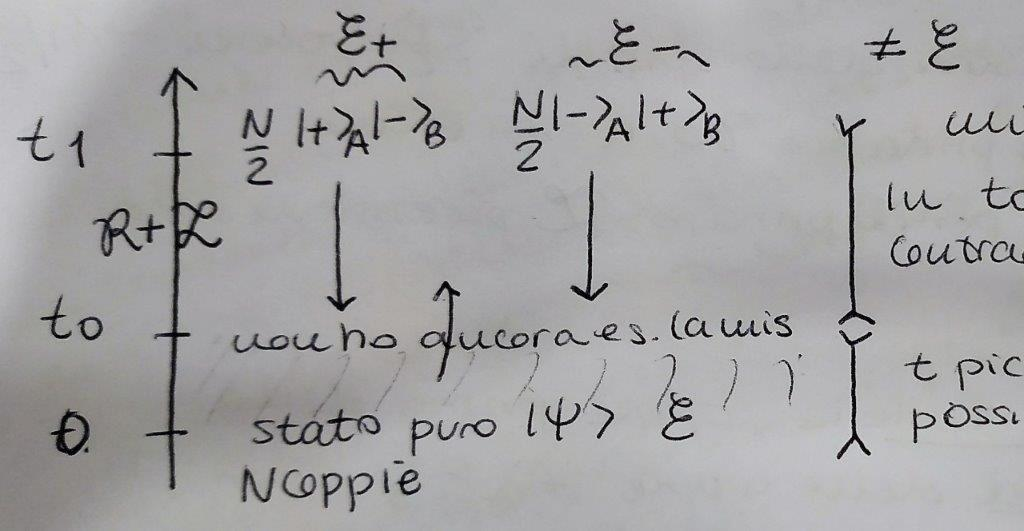
\includegraphics[scale=0.4]{Immagini/19_12/image001.jpg}
\caption{L'incompatibilità tra $\mathcal{R}, \mathcal{L}$ e $\mathcal{C}$}
\end{figure}

\begin{comment}
In $t_1$ abbiamo fatto una misura che \textit{non può disturbare} $B$, dato che $A$ e $B$ sono a distanza di tipo spazio, e da cui ricaviamo informazione su $B$. Ma allora, per $\mathcal{R}$, l'informazione ottenuta \q{senza disturbare $B$} è una \textit{proprietà oggettiva} di $B$, ovvero anche se non avessimo misurato $A$, $B$ avrebbe avuto tale proprietà.\\
Per esempio, se su $A$ ricaviamo $\hbar/2$, sappiamo che da $B$ otterremo $-\hbar/2$, \textit{senza misurarlo}. Ma allora, per $\mathcal{R}$, significa che anche se non avessimo misurato $A$, $B$ sarebbe stato in $-\hbar/2$.\\
Per $\mathcal{L}$ possiamo\footnote{$\mathcal{L}$ riguarda solo le \textit{proprietà oggettive}, e perciò questo possiamo farlo solo perché per $\mathcal{R}$ sappiamo che il risultato su $B$ è una \textit{proprietà oggettiva}.} \q{trasportare} tale risultato per tutto l'intervallo temporale in cui siamo sicuri che le due particelle \textit{non possano interagire}, ossia da $t_0$ all'istante di misura $t_1$, dove $t_0$ è definito come l'istante in cui le due particelle si trovano a distanza di \textit{tipo spazio}.\\
Ora, per $\mathcal{C}$ sappiamo che $\ket{\psi}$ descrive \q{completamente} il sistema. Ma allora, per evoluzione unitaria, $\ket{\psi}$ rimane la stessa (a meno di una fase) fino alla misura, ossia tra $0$ e $t_1$.\\
Ma allora sorge una contraddizione: tra $t_0$ e $t_1$ lo stato deve essere per tutte le $N$ $\ket{\psi}$, ma \textit{anche} $\ket{+}_A \ket{-}_B$ per $N/2$ particelle e $\ket{-}_A \ket{+}_B$ per l'altra metà.\\
Ciò costituisce, essenzialemente, il nucleo del paradosso EPR.\\
\end{comment}

\subsection{Risolvere il paradosso}
Abbiamo allora $3$ possibilità \q{minimali} per risolvere la situazione, che corrispondono a rinunciare a uno dei tre principi: $\mathcal{R}$, $\mathcal{L}$ o $\mathcal{C}$ (trascuriamo, per ora, il caso \textit{brutto} in cui dovremmo rinunciare a \textit{più di un} principio).\\

\begin{itemize}
\item \textbf{Rinunciamo a} $\mathcal{R}$ (ovvero a CFD) dichiarando che anche sapendo con certezza il valore che si otterrebbe misurando un'osservabile \textit{senza} disturbare il sistema, a questo valore \textit{non} si può attribuire il carattere di una proprietà fisica oggettiva indipendente dalla misura. Non possiamo in particolare estrapolare l'informazione prima della misura, anche conoscendo la dinamica del sistema. In tal modo non possiamo \q{portare indietro} il risultato ottenuto in $t_1$, e quindi non si ha contraddizione in $[t_0, t_1]$.\\
L'abbandonare $\mathcal{R}$ significa in sostanza sostenere che la funzione d'onda non è una proprietà del sistema fisico indipendente dall'osservazione, neppure per gli autostati, ma è un oggetto matematico che sintetizza un insieme massimale di informazioni sul sistema. La \MQ è perciò un paradigma che consente di conoscere l'evoluzione temporale dell'informazione e di fare predizioni sui risultati (\textit{strumentalismo} per gli stati $\psi$).\\
$\mathcal{L}$ è allora preservato dal fatto che le osservazioni modificano le nostre \textit{conoscenze sui sistemi}, ma non le loro proprietà \textit{oggettive} (di cui $\psi$ non fa più parte). Perciò a cambiare sono le predizioni, anche nel caso di conoscenza massimale, analogamente a quanto succede in \MC quando si ha conoscenza non massimale.\
\textit{Si potrebbe dire che la misura \q{crea} lo stato}.
\item Rinunciamo a $\mathcal{L}$. Osserviamo che se ora applichiamo $\mathcal{R}$, lo stato diventa una \textit{proprietà oggettiva}. Infatti $\ket{\psi}\bra{\psi}$ è un'osservabile, e supponendo di produrre lo \textit{stesso} sistema \textit{più volte} nello stato $\ket{\psi}$ (incognito), misurando i suoi elementi di matrice possiamo determinarlo esattamente (nel caso in esame con $4\times 4$ misure, effettuate con tecniche di \textit{tomografia quantistica}) lasciando le altre coppie senza disturbo. Secondo $\mathcal{R}$ senza $\mathcal{L}$ una misura può modificare \textit{istantaneamente} la funzione d'onda a distanze arbitrariamente grandi. Non si può perciò prolungare all'indietro l'informazione neppure se i sistemi sono a distanze di tipo spazio, dato che anche in tal caso potrebbero, in principio, influenzarsi a vicenda: in altre parole non esiste più un $t_0$ dopo il quale i due sistemi sono completamente non interagenti.\\
Fortunatamente si può dimostrare che, usando tali modifiche, non si possono trasmettere informazioni \textit{più velocemente} di $c$. Infatti, poiché ogni misura trova in maniera \textit{casuale} uno dei due risultati, $B$ vede una sequenza casuale di $+$ e $-$, che senza l'informazione su $A$ è \textit{perfettamente compatibile,} ad esempio, con l'eventualità in cui su $A$ non è stata fatta alcuna misura. Solo quando $A$ e $B$ \textit{confrontano} le loro misure è possibile notare che ogni $+$ di $A$ corrisponde a un $-$ di $B$, e quindi si nota la correlazione. Ma per avere l'informazione che rivela la correlazione a distanze di tipo spazio $A$ deve inviare un'informazione a $B$, e tale comunicazione è per forza limitata da $c$.\\
Perciò, anche rinunciando a $\mathcal{L}$ vale ancora la relatività, e la causalità è salva.\\
Il realismo $\mathcal{R}$ può essere mantenuto abbandonando il \textit{riduzionismo}, che sostiene che un sistema è semplicemente la somma dei suoi costituenti. Senza $\mathcal{L}$, infatti, il risultato di un esperimento dipende non solo dai suoi costituenti, ma potenzialmente dallo stato di tutto l'universo, e la realtà diventa una \textit{foresta di funzioni d'onda entangled}.
\item Rinunciamo a $\mathcal{C}$ (posizione sostenuta da Einstein). Il fatto che (per $\mathcal{R} + \mathcal{L}$), dopo la misura di spin di $A$, gli spin di $B$ \q{abbiano} individualmente valore $+\hbar/2$ o $-\hbar/2$ \textit{senza} che siano stati disturbati può far supporre che tale proprietà l'avessero anche \textit{prima} della misura (esattamente come il colore delle palle classiche), solo che la $\ket{\psi}$, che è la stessa per tutte le coppie prima della misura, semplicemente \textit{non aveva} quest'informazione. \textit{In altre parole, gli spin di $A$ e $B$ erano già definiti in precedenza, ma non erano conoscibili tramite $\ket{\psi}$, che quindi costituiva un'informazione incompleta del sistema}.\\
Quindi la $\psi$ dà solo informazioni probabilistiche come \textit{media} di \textit{variabili \q{nascoste}} che costituiscono le \q{vere} variabili reali.\\
\textit{Un'analogia è la temperatura in Meccanica Statistica, che è semplicemente una media su un numero molto grande di particelle, i cui stati non sono misurati individualmente}.\\
\end{itemize}




\begin{comment}
\section{Appunti Nicrosini}
\textbf{Non separabilità} Quando due sistemi quantistici, ciascuno dei quali sia originariamente caratterizzato da un insieme competo di proprietà definite, una volta che abbiano interagito non è più possibile, in generale, pensare a ciascuno di essi come dotato di un insieme completo di proprietà definite, dove per \q{proprietà definite} si intendono esattamente valori specifici delle osservabili associate solamente a quel sistema e indipendenti da futuri esperimenti sul sistema stesso.\\
Tale conclusione continua a valere anche per sistemi che abbiano interagito ma che non interagiscano più al tempo in cui vengano considerati.\\

In altre parole: consideriamo due sistemi $U$ e $V$. Separatamente i due, all'inizio, si trovano in stati ben definiti per certe osservabili. Dopo l'interazione non sono più considerabili separabili, in quanto \q{intrecciati}.\\

Teoria completa = ogni suo elemento corrisponde ad un elemento di realtà.\\
In \MQ: osservabili che non commutano non sono misurabili contemporaneamente.\\
Due possibilità:
\begin{itemize}
\item O le due osservabili sono \q{reali}, cioè hanno un valore ben definito, che però non è contemplato dalla \MQ, che quindi è incompleta
\item Oppure le due osservabili non sono entrambe reali allo stesso tempo
\end{itemize}
Tuttavia, consideriamo due oggetti lontani, che non possono interagire tra loro. Se la \MQ è completa, e i due oggetti sono entangled, non possiamo misurare entrambe le proprietà, che quindi non sono reali. Ma i due oggetti sono lontani e non possono interagire, quindi devono avere proprietà reali, da cui la contraddizione.\\

Distinzione tra \textbf{realtà oggettiva} e i \textbf{concetti fisici} che usiamo per descriverla.\\
La validità di una teoria è data dalla sua \textbf{correttezza}, cioè dall'accordo con gli esperimenti, e \textbf{completa}, se \q{acconta per tutto ciò che fa parte della realtà oggettiva}, ossia ogni elemento della realtà fisica deve avere una controparte nella teoria fisica.\\
Per capire se una teoria è completa o meno, dobbiamo determinare gli \textit{elementi di realtà}. Poiché siamo in fisica, dovremo farlo non \textit{a priori}, ma tramite esperimenti e misurazioni. Ci accontentiamo perciò di una condizione sufficiente: \textit{se, senza disturbare in nessu nmodo un sistema, possiamo perevedere con certezza (cioè con probabilità unitaria) il valore di una quantità fisica, allora esiste un elemento di realtà fisica corrispondente a questa quantità fisica}.\\
Esempio: se una particella è in un autostato dell'osservabile $A$ con autovalore $a$, cioè se vale:
\begin{align*}
A\psi = a \psi
\end{align*}
allora c'è un elemento di realtà fisica corrispondente alla quantità $A$, poiché \textit{anche senza misurare} sappiamo che una misura di $A$ restituirebbe un valore definito $a$ (definitezza controfattuale).\\

Sappiamo che se due operatori $A$ e $B$ non commutano, allora la conoscenza precisa di una preclude la conoscenza dell'altra.\\
Abbiamo due possibilità:
\begin{itemize}
\item Ad $A$ e $B$ corrispondono due elementi di realtà. Ma allora una teoria completa dovrebbe essere in grado di predirli, e poiché così non succede in \MQ, si ha che la \MQ è incompleta.
\item Se invece $A$ e $B$ non possono essere contemporaneamente reali, si ha che la \MQ descrive completamente la situazione.
\end{itemize}

\end{comment}
\end{document}

